%%%%%%%%% JPS abstruct %%%%%%%%%%%%%%%%%%%%%%%%%%%%%%%%%%%%%%%%%%
\documentclass[12pt,a4paper]{jsarticle}

%%%%%%%%% packages %%%%%%%%%%%%%%%%%%%%%%%%%%%%%%%%%%%%%%%%%%%%%%
\usepackage[dvipdfmx]{graphicx} % Include figure files
\usepackage[%                           % 余白の設定
%mag=1400,%                              jarticle の場合(14pt)に
dvipdfm,truedimen,%
top=30truemm,bottom=20truemm,%
left=20truemm,right=20truemm]{geometry}
\usepackage{array,booktabs}
\usepackage{float}
\usepackage{wrapfig}
\usepackage[hang,small,bf]{caption}
\usepackage[subrefformat=parens]{subcaption}
\captionsetup{compatibility=false}

\pagestyle{empty}

%%%%%%%%% header %%%%%%%%%%%%%%%%%%%%%%%%%%%%%%%%%%%%%%%%%%%%%%%%
\begin{document}
\vspace{-5pt}
\begin{center}
  {\gt \Large ニューラルネットワークを用いたTPCの飛跡検出法の開発 }\\[14pt]
  
  {\gt \large 京大理$^{\rm{A}}$ 阪大理$^{\rm{B}}$ 阪大RCNP$^{\rm{C}}$\\
    土井隆暢$^{\rm{A}}$, 川畑貴裕$^{\rm{B}}$, 古野達也$^{\rm{C}}$}\\[5pt]
  
  {\large \bf Development of analysis method for TPC track \\
    using neural network.}\\[5pt]
  
  {\large \it $^{\rm{A}}$Dep. of Phys., Kyoto Univ. $^{\rm{B}}$Dep. of Phys., Osaka Univ. \\
    $^{\rm{C}}$RCNP, Osaka Univ.}\\
  
  {\large \bf T. Doi$^{\rm{A}}$, T. Kawabata$^{\rm{B}}$, and T. Furuno$^{\rm{C}}$}
\end{center}

\vspace{5pt}
%%%%%%%%% main %%%%%%%%%%%%%%%%%%%%%%%%%%%%%%%%%%%%%%%%%%%%%%%%%%

\begin{wrapfigure}{r}{20zw}
  \vspace*{-1\intextsep}
  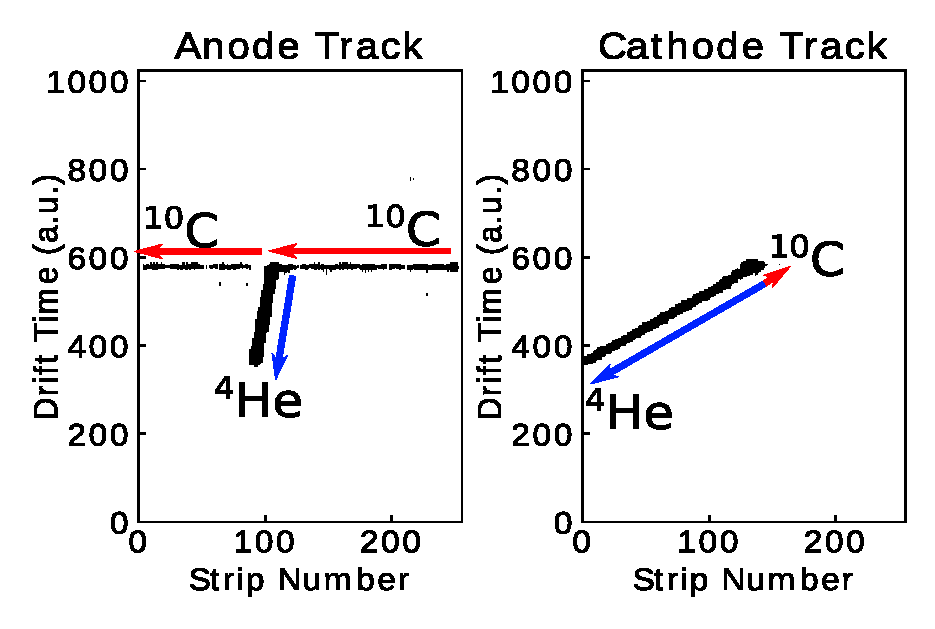
\includegraphics[clip,width=20zw]{true.eps}
  \caption{
    MAIKo TPC を用いて測定される${}^{10}\rm{C} + {}^{4}\rm{He}$散乱事象の飛跡データ。
    左がビームに平行な面、右がビームに垂直な面に
    飛跡を射影した画像。
  }
  \label{fig:track}
\end{wrapfigure}MAIKo TPC% (Mu-PIC based Active target for Inverse Kinematics .)
は荷電粒子の飛跡を三次元的に測定出来るガス検出器であり、
検出器中のガスを標的として用いることで、
従来の標的では実現できない低エネルギー粒子の測定が可能となる。
図\ref{fig:track}%ような画像データが得られる。
に示すように、MAIKo TPC からは
3次元の飛跡をビーム入射方向に対して平行な面に射影した飛跡と
ビーム入射方向に対して垂直な面に射影した飛跡の
2つの2次元画像が得られる。
取得された画像データから散乱角度や励起エネルギーなどの
情報を得るためには、
画像解析を行って飛跡の方向と長さを抽出する必要がある。

我々はこれまでHough 変換により飛跡の長さと方向を決定していた。
しかし、この解析にはHough 変換を用いた複雑なアルゴリズムが必要であった。
そこで、我々はHough 変換を用いた従来手法に代わる新たな手法として、
ニューラルネットワークを用いたアルゴリズムの開発を行っている。
すでに、実際の測定データを用いてニューラルネットワークを学習させ、
従来手法より高速に飛跡の長さや方向を抽出することに成功している。
高速に解析を行えるニューラルネットワークを用いれば、
測定中にリアルタイムでオンライン解析することが可能となるが、
そのためには学習データを実験前に用意しなければならず、
実際の測定データを学習データに用いることができない。
そこで、現実的な測定条件を考慮したシミュレーションを行うことで、
実験前に学習データの生成およびニューラルネットワークの学習を行えば、
新手法によるオンライン解析が可能となる。

本講演では、シミュレーションによる疑似データで学習させた
ニューラルネットワークによる飛跡情報の抽出結果について報告する。

%\begin{figure}[h]
%\end{figure}

\end{document}
